\documentclass[11pt]{article}

\usepackage[T1]{fontenc}
\usepackage[utf8]{inputenc}
\usepackage{lmodern}
\usepackage[margin=1in]{geometry}
\usepackage{microtype}
\usepackage{amsmath}
\usepackage{booktabs}
\usepackage{tabularx}
\usepackage{xcolor}
\usepackage{listings}
\usepackage{tikz}
\usetikzlibrary{positioning,arrows.meta,fit,backgrounds}
\usepackage[numbers,sort&compress]{natbib}
\usepackage[hidelinks]{hyperref}
\usepackage{cleveref}
\hypersetup{pdfauthor={dgxcoder}, pdftitle={Mightling: A Vendor-Free Coding Agent on a Single Unified-Memory Workstation}}

\lstset{
  basicstyle=\ttfamily\small,
  columns=fullflexible,
  keepspaces=true,
  breaklines=true,
  frame=single,
  framerule=0.3pt,
  xleftmargin=0.5em,
  xrightmargin=0.5em,
}

\newcommand{\code}[1]{\texttt{#1}}

\title{Mightling: A Vendor-Free Coding Agent on a Single Unified-Memory Workstation, Built on
the Codex CLI}

\author{dgxcoder\\ \texttt{dgxcoder@dreamference.ai}}

\date{October 2026}

\begin{document}
\maketitle

\begin{abstract}
Terminal coding agents such as the Codex CLI are open source, but they are built around a
hosted model, a vendor account and a cloud of companion services. We describe \emph{Mightling}, a
coding agent whose model runs on one NVIDIA GB10 workstation (128\,GB of CPU--GPU unified memory):
a 27B-parameter hybrid Gated-DeltaNet/Transformer model (Qwen3.8-27B, NVFP4) served locally through
SGLang or an opt-in model-specific C++/CUDA engine (\code{ling-serve}) with a calibrated NVFP4
DFlash2 block-diffusion drafter. Source code, prompts and inference never leave the machine, and no
vendor account is involved. Mightling is a fork of the Codex CLI (release \code{rust-v0.158.0},
4{,}894 Rust source files, 1.93 million lines). Its central engineering choice is to keep the fork
almost identical to upstream. The upstream tree is never edited. Each build exports it, applies a
series of 32 patches totalling 57.6\,KB (57{,}571 bytes across 62 files, $+255/-89$ lines), and
links in a separate workspace of crates (94.0k lines of Rust) that does the actual work of
localisation and extension: model discovery, configuration, prompt rebranding, help-text rewriting,
a signed release-based updater and refusal of cloud-bound commands. De-vendoring and localisation
take 29.1\,KB (16 patches, down from 406\,KB before runtime rebranding); the other 16 patches
(28.5\,KB) are one- and two-line hooks for local features and platform sandboxing. We describe the
inventory of cloud dependencies that are switched off, the trace-based egress audit that keeps them
off, an enforced air-gap switch that also masks host control sockets, the protocol and caching
traps between a vendor harness and a local model server, and the host-safety layer that unified
memory requires when CUDA allocations bypass container cgroups. On a 100-task sample of SWE-bench
Verified, run inside each task's container on this machine, a single attempt resolves 68;
calibrated against 175 published leaderboard submissions on the same tasks, that corresponds to
about 69\% on all of Verified (95\% band 64--73\%). A two-session ``study, then fix'' mode resolves
69 of the same 100 at $2.2\times$ the time, and five single-attempt prompt and harness changes on
44--50 tasks lie within single-run variance (three runs of the default arm on 44 tasks resolve 29,
29 and 31, with 36 solved by at least one). Multi-attempt selection clears that noise: a two-stage best-of-3 chooser (regression test filter
plus pairwise diff judge) resolves 33 of those 44 tasks offline and, live, 31 of 50 against 22 of
50 for the first of its three single runs (exact paired test, $p = 0.022$). On one 50-task night,
\code{ling-serve} resolves 33 against SGLang's 29, in 4\,h\,28\,min instead of 7\,h\,32\,min. We discuss threats
to validity and what remains unmeasured.
\end{abstract}

\section{Introduction}

Agentic coding tools now read repositories, run shell commands and edit files autonomously
\cite{yao2023react,yang2024sweagent,wang2024openhands}. The most capable are open-source clients of
proprietary services: the client is inspectable, but a session sends source code, prompts and tool
output to a hosted model, which regulated industries, security research and anyone whose code is
the asset cannot accept. Two developments make a local alternative plausible: open-weight models
quantised to four bits \cite{frantar2022gptq,lin2023awq,cheng2023autoround,nvfp4blog} with
speculative decoding \cite{leviathan2023speculative,chen2023speculative,chen2026dflash} generate at
interactive speed on one desk-side machine, and the leading agent clients are open source, so a
local deployment can reuse their tool-calling loop, sandboxing, approval flows and terminal UI.
Reusing a fast-moving upstream has a cost: a fork that edits freely soon cannot take upstream
releases, and one that edits nothing cannot remove the parts that assume a cloud. This paper
describes how Mightling, a local AI stack for the NVIDIA GB10 made by Dreamference, resolves that
tension in its terminal coding agent, \code{ling}.

\paragraph{What ``local'' means here.} The model, the agent and all session state run on one
workstation; source code, prompts, tool output and model traffic never leave it, and a traced
session shows no connection to any vendor (\cref{sec:egress}). Mightling is not air-gapped by
default: web search goes through a SearXNG \cite{searxng} instance on the machine, mail is read
over IMAP, \code{ling update} contacts GitHub, and optional phone messengers reach
their networks once turned on. Each can be switched off, and \code{/airgapped on} gives every
sandboxed command an empty network namespace and masks the host's control sockets (\cref{sec:egress}).

\paragraph{Contributions.}
\begin{enumerate}
\item A \textbf{patch-minimal fork architecture} for a 1.93M-line Rust agent (\cref{sec:fork}): an
unmodified pinned submodule, a build-time export, one- and two-line hooks, and an external crate
linked into the binary, with four techniques that keep the entire 32-patch series at 57.6\,KB
(29.1\,KB for de-vendoring and localisation, 28.5\,KB for features and platform hooks) while passing
21{,}413 of 21{,}414 upstream tests on the patched tree.
\item An \textbf{inventory of the cloud surface} of a production coding-agent client and its
treatment (\cref{sec:cloud}), a \code{strace}-based egress audit run after every build, and a
sandbox-enforced air-gap switch with explicit analysis of host-socket and \code{git}-config
boundaries.
\item \textbf{Empirical findings at the harness--server boundary} (\cref{sec:local}): tool types
that local servers silently drop (\code{namespace} MCP tools and \code{custom} grammar tools),
\code{/v1/responses} history-reconstruction and streaming bugs in SGLang, patched at launch (the
benchmark nights on the affected release resolved 40--52\% against 62--74\% before it), a compaction prefix-cache invalidation bug
where omitting tool schemas forced 62--91k-token cold re-prefills, a KV-pool-tied compaction limit
with turn-end compaction and a rule-built state ledger, a streaming repetition loop guard, and a
measured output cost model.
\item A \textbf{host-safety layer for unified memory} (\cref{sec:safety}) addressing direct-reclaim
livelocks and CUDA allocations that bypass container cgroup accounting.
\item A \textbf{task-level evaluation on SWE-bench Verified} on arm64 (\cref{sec:swebench}) with a
calibrated overall estimate, a failure and test-regression taxonomy, a statistical power analysis
of single-attempt A/B nights ($N=44$--$50$), a significant gain from a two-stage best-of-3 chooser
($p = 0.022$), and a first end-to-end comparison of our model-specific C++/CUDA engine
\code{ling-serve} against SGLang (\cref{sec:engine}).
\end{enumerate}

\section{Background}

\paragraph{The Codex CLI.} The Codex CLI \cite{openai2026codex} is an open-source Rust workspace of
about 160 crates: a terminal UI, a non-interactive \code{exec} mode, an \code{app-server} speaking
JSON-RPC over stdio, session resume and fork, a platform sandbox (Bubblewrap \cite{bubblewrap2024}
on Linux) and an approval model for tool calls. In \emph{Code Mode} the model is given a single
\code{exec} tool and writes short JavaScript programs, run by a separate V8 host process
(\code{codex-code-mode-host}), within which every other tool, including Model Context Protocol
(MCP) \cite{mcp2025spec} tools, is a callable function. Codex talks to open-source providers
(\code{-{}-oss}) through the \code{/v1/responses} endpoint, but login, cloud tasks,
connectors, usage limits, telemetry and feedback upload assume an account with the vendor's hosted
service.

\paragraph{The machine.} The NVIDIA GB10 pairs a 20-core Arm CPU (\code{aarch64}) with a Blackwell
GPU (compute capability SM121) over 128\,GB of shared LPDDR5X at roughly 273\,GB/s. No memory is
reserved for the GPU: model weights, KV cache, the desktop and every other process draw from one
pool, which shapes \cref{sec:safety}.

\paragraph{The model and engines.} Mightling serves one default model: Qwen3.8-27B \cite{qwen3tr}
(48 Gated DeltaNet linear-attention layers \cite{yang2024deltanet,yang2025gateddeltanet} and 16
full-attention layers, 64 layers in all) in an NVFP4 checkpoint \cite{nvfp4blog,ocpmx2023}, paired
with a calibrated NVFP4 DFlash2 block-diffusion drafter \cite{chen2026dflash,dflash2drafter}
(Dreamference's ScaleSearch block-scale quantisation from release 1.7.2, replacing an earlier RTN
build) at a 262{,}144-token context window, leaving about 38.7\,GB of host memory free while
serving. By default it runs on SGLang \cite{zheng2023sglang} (pinned at v0.5.21). On the benchmark
prompts of \path{scripts/decode_speed.py} at 12 draft tokens, single-stream greedy decoding reaches
32.0, 68.6 and 84.1 tokens/s on prose, code and JSON (accepting 3.4, 4.4 and 5.9 draft tokens per
step, with prefill at 1{,}805 tokens/s on 13.2k tokens; an earlier 16-token recipe on unrecorded
prompts measured 25.5, 50.3 and 87.0 tokens/s and 1{,}688 tokens/s prefill, ~1{,}004 tokens/s at
116k). On replayed agent sessions, 12 draft tokens beat 16 by 7\% single-stream (48.3 against
45.1 tokens/s, 5.23 against 4.99 accepted tokens per ~103\,ms step) and tied on two concurrent
streams (33.9 tokens/s per stream). Since release 1.7.2, the same checkpoint and drafter can also
be served opt-in by \code{ling-serve} (\cref{sec:engine}), our model-specific C++/CUDA engine; the
server manager also retains its vLLM \cite{kwon2023vllm} launch path for candidate trials.

\section{System overview}
\label{sec:overview}

\begin{figure}[t]
\centering
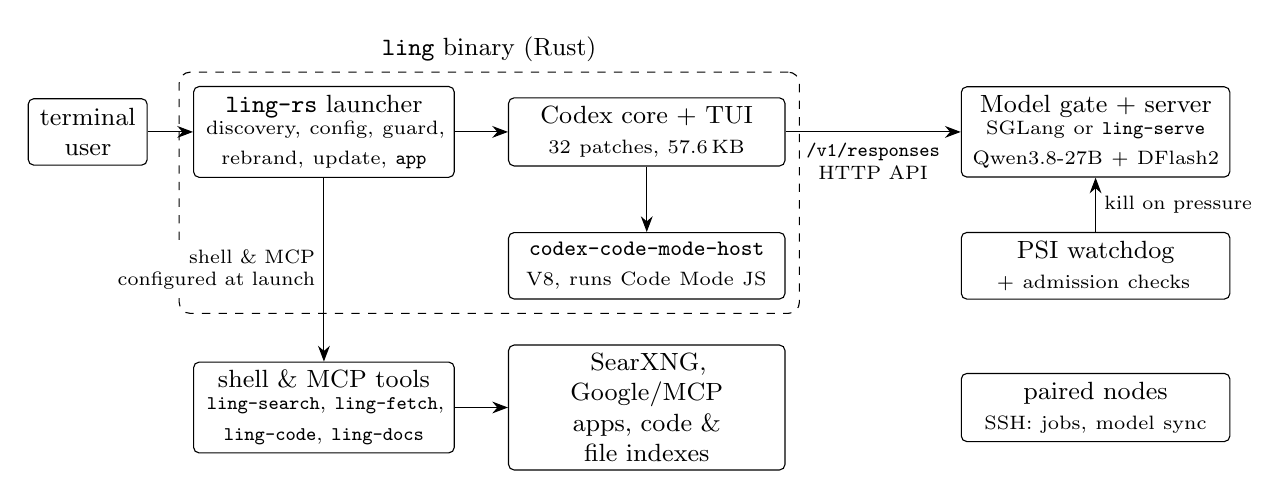
\begin{tikzpicture}[
  box/.style={draw, rounded corners=2pt, align=center, font=\small, inner sep=3pt,
              minimum height=2.4em, text width=#1},
  box/.default=2.6cm,
  grp/.style={draw, dashed, rounded corners=4pt, inner sep=5pt},
  lbl/.style={font=\scriptsize, fill=white, inner sep=1pt},
  >={Stealth[length=2mm]}]
  % row 1: the request path
  \node[box=1.3cm]  (user)     at (-0.2,0)  {terminal\\user};
  \node[box=3.1cm]  (launcher) at (2.8,0)   {\code{ling-rs} launcher\\\scriptsize discovery, config, guard,\\rebrand, update, \code{app}};
  \node[box=3.3cm]  (codex)    at (6.9,0)   {Codex core + TUI\\\scriptsize 32 patches, 57.6\,KB};
  \node[box=3.2cm]  (vllm)     at (12.6,0)  {Model gate + server\\\scriptsize SGLang or \code{ling-serve}\\Qwen3.8-27B + DFlash2};
  % row 2
  \node[box=3.3cm]  (host)     at (6.9,-1.7)  {{\footnotesize\code{codex-code-mode-host}}\\\scriptsize V8, runs Code Mode JS};
  \node[box=3.2cm]  (watch)    at (12.6,-1.7) {PSI watchdog\\\scriptsize + admission checks};
  % row 3
  \node[box=3.1cm]  (tools)    at (2.8,-3.5)  {shell \& MCP tools\\\scriptsize\code{ling-search}, \code{ling-fetch},\\\code{ling-code}, \code{ling-docs}};
  \node[box=3.3cm]  (svc)      at (6.9,-3.5)  {SearXNG, Google/MCP\\apps, code \& file indexes};
  \node[box=3.2cm]  (diff)     at (12.6,-3.5) {paired nodes\\\scriptsize SSH: jobs, model sync};
  % the binary
  \begin{scope}[on background layer]
    \node[grp, fit=(launcher)(codex)(host), label={[font=\small]above:\code{ling} binary (Rust)}] {};
  \end{scope}
  \draw[->] (user) -- (launcher);
  \draw[->] (launcher) -- (codex);
  \draw[->] (codex) -- (host);
  \draw[->] (codex) -- node[lbl, below=3pt, align=center] {\code{/v1/responses}\\HTTP API} (vllm);
  \draw[->] (watch) -- node[lbl, right=2pt] {kill on pressure} (vllm);
  \draw[->] (launcher) -- node[lbl, left=2pt, align=right] {shell \& MCP\\configured at launch} (tools);
  \draw[->] (tools) -- (svc);
\end{tikzpicture}
\caption{Mightling at run time. The only Codex code paths that differ from upstream are the hooks
applied by the 32-patch series; everything Mightling-specific lives in the linked \code{ling-rs}
workspace or in separate local binaries and services.}
\label{fig:overview}
\end{figure}

\Cref{fig:overview} shows the running system. The user types \code{ling}, a single Rust binary.
Before Codex parses its command line, the linked launcher crate finds the local model server (via
environment, configuration, node ID or mDNS) and waits for it if it is still loading, queries
\code{/v1/models} for the served model ID, context length and any verified LoRA adapters, writes
the model catalogue and configuration Codex needs, and prepends the options that point Codex at the
local provider. From then on the process is Codex, and every upstream flag and subcommand behaves
as documented, apart from the cloud surfaces of \cref{sec:cloud}. Four standalone Rust binaries
beside \code{ling} provide web search, page fetching, repository code navigation and local document
search (\code{ling-search}, \code{ling-fetch}, \code{ling-code}, \code{ling-docs});
\code{ling-admin}, the Python management CLI, manages the model-server container and its streaming
model-gate proxy, the Google service (Gmail, Drive, Calendar), image-search and voice sidecars, the
overnight queue, workstation pairing, SWE-bench runs and the build of \code{ling}. A built-in Rust
web server (\code{ling web}) and an Electron desktop app (\code{ling app}, replacing an earlier
Onyx-based browser chat \cite{onyx} retired in release 1.7.0) share the same \code{ling app-server}
backend (\cref{sec:rest}).

\section{A patch-minimal fork}
\label{sec:fork}

\subsection{Build and verification pipeline}

Codex is vendored as a git submodule of our own GitHub fork, pinned to the stable release tag
\code{rust-v0.158.0}, and \emph{never modified}: the builder's tests assert that \code{git status}
inside it is empty after a build. A build takes an exclusive file lock, exports the pinned
\code{codex-rs/} with \code{git archive}, copies the launcher workspace in as \code{codex-rs/ling},
applies the patch series with \code{git apply -{}-check} before \code{git apply} so a stale patch
fails before anything is half-applied, stamps Mightling's release version into the exported
workspace manifest, builds \code{ling} and \code{codex-code-mode-host} with Cargo (using
\code{sccache} when present), installs them side by side, records a content-addressed build key so
an unchanged tree skips the build, and runs the network egress audit (\cref{sec:egress}). Moving to
a new upstream release is designed to mean bumping the submodule tag and refreshing whichever hunks
stop applying; because the hunks are one- and two-line hooks, conflicts are local, although we note
in \cref{sec:limits} that this fork has so far tracked a single pinned release tag.

To verify that the patches do not break upstream behaviour, \code{ling-admin codex test} runs
Codex's own Rust test suite against a separate export of the patched tree inside a 24\,GiB
memory-capped systemd scope. Rather than skipping the ~130 TUI snapshot tests that check the
on-screen product name, the runner overlays Mightling's accepted \code{.snap} files
(\path{codex-tests/snapshots/}, checked by a width-preservation test so box borders never drift)
and six small test-only adaptation diffs (\path{codex-tests/patches/}). On the 31-patch tree
(2026-10-27), 21{,}414 upstream tests ran: 21{,}413 passed and 234 were skipped on a documented
skip list (\path{codex-tests/mightling-skips.toml}) where each entry is verified by leaving its
patch out of the tree (for example, 16 app-server tests that timed out in early runs were proved on
2026-10-02 to wait for analytics events that patch 0013 disables, and pass in 46\,s when 0013 is
omitted).

\subsection{Four techniques keep the series small}

\Cref{tab:patches} lists the 32 patches. \emph{Rename at run time, not in the tree}: renaming the
agent inside Codex's bundled model catalogue would cost about 395\,KB of diff, since each 20\,KB
system-prompt template is one JSON line (our initial pre-minimisation patch series was 406.1\,KB);
the launcher instead reads the catalogue through the upstream crate's public function, replaces the
identity sentence, and hands the result to Codex in the catalogue it writes anyway. \emph{Rewrite
presentation where it is assembled}: one hook routes argument parsing through a launcher function
that walks the \code{clap} tree once and rewrites the product name in every \code{about},
\code{help} and \code{bin\_name}. \emph{Use the build system's own unification}: one
\code{openssl-sys = \{features = ["vendored"]\}} line in \emph{our} manifest applies to every crate
that links OpenSSL, and a path dependency inside the workspace root makes the launcher a workspace
member without editing the workspace manifest. \emph{One line per behaviour}: what remains is a
\code{false} from a visibility predicate, a \code{hide = true}, or a dispatch arm sent into the
launcher.

\paragraph{De-vendoring versus features.} The initial branding and launcher hook (\code{0001} and
\code{0002}) take 8.2\,KB (about 9\,KB in the first four-patch series). Together with the
cloud-surface switches (\code{0005}--\code{0016}), neutral vendor wording across plugin and
connector screens (\code{0030}) and Windows doctor checks (\code{0034}), the 16 de-vendoring and
localisation patches total 29.1\,KB (29{,}076 bytes). The remaining 16 patches (28.5\,KB, 28{,}495
bytes) are features and sandbox/platform hooks, each with its logic in a crate of ours and only its
entry point in Codex: \code{/night} (\code{0018}), \code{/airgapped} on Linux, the app server and
Windows (\code{0019}, \code{0023}, \code{0024}, \code{0031}), flattening MCP tools and translating
Code Mode's \code{exec} (\code{0020}), observation masking and drop-first compaction (\code{0021},
\code{0026}), cache-hot compaction tool lists (\code{0027}), local \code{/apps} connectors
(\code{0022}), \code{/node} (\code{0025}), \code{/adapter} (\code{0028}), Claude Code
compatibility hooks and fail-closed guard (\code{0029}, \code{0032}), and Windows/symlink runtime
fixes (\code{0033}, \code{0035}). A test caps the series at 64\,KB, raised only explicitly when a
new hook is approved (an experimental terse-answer hook, \code{0017-cave-mode}, was removed on
2026-10-28; \cref{sec:local}). Two build details need no patch: Code Mode's V8 flavour is not
published by \code{denoland} for \code{aarch64-unknown-linux-gnu}, so the builder fetches
upstream's own prebuilt archive and verifies it against the submodule's SHA-256 manifest
\cite{rustyv8}, and two release-profile environment overrides strip debug line tables to take the
binary from 1.4\,GB to 315\,MB.

\begin{table}[tbp]
\centering
\scriptsize
\begin{tabularx}{\linewidth}{@{}l r r X@{}}
\toprule
Patch & Files & $+/-$ & Purpose \\
\midrule
0001 brand-mightling-name & 12 & 24/24 & Product name in TUI header, status card, command popup, \code{exec} banner, usage and resume lines \\
0002 ling-launcher-hook & 2 & 2/1 & One dependency line; route argv through the launcher and parse-time help rebrander \\
0005 hide-vendor-login & 2 & 4/0 & Hide \code{login}/\code{logout} and \code{/logout} \\
0006 hide-cloud & 1 & 2/1 & Hide \code{cloud} (kept compiled for a future private cloud) \\
0007 hide-remote-control & 1 & 2/0 & Hide \code{remote-control} \\
0008 mightling-update & 1 & 2/2 & Send \code{update} to the launcher's Ed25519-verified release updater \\
0009 remove-feedback & 2 & 3/1 & Remove \code{/feedback} (uploads session logs) \\
0010 hide-voice & 1 & 4/1 & Hide \code{/voice} (hosted realtime API) and \code{/pets} (art fetched from vendor CDN) \\
0011 usage-token-stats & 4 & 7/17 & \code{/usage} shows local session token statistics \\
0012 hide-auto-review & 1 & 4/0 & Hide \code{/approve} (hosted review model) and \code{/import} (untraced GitHub plugin fetch) \\
0013 disable-usage-analytics & 1 & 2/1 & Construct the analytics client disabled \\
0014 mightling-home & 1 & 2/0 & Use \code{\textasciitilde/.mightling}, never upstream's shared login folder \\
0015 no-vendor-network & 4 & 20/4 & Close the four login-free channels found by tracing (\cref{sec:egress}) \\
0016 doctor-offline & 2 & 20/0 & Switch off \code{doctor}'s sign-in, update and reachability checks \\
0018 night-slash-command & 2 & 7/0 & \code{/night}: queue or apply an overnight task (\cref{sec:rest}) \\
0019 airgapped & 9 & 21/3 & \code{/airgapped}; empty network namespace and mask host control sockets at \code{on}; refuse Full Access \\
0020 flat-mcp-tools & 3 & 4/1 & Send MCP tools and Code Mode's \code{exec} as plain functions (\cref{sec:local}) \\
0021 observation-masking & 2 & 5/1 & Optionally replace old tool outputs by a placeholder naming a saved copy \\
0022 ling-apps & 2 & 6/1 & \code{/apps} lists local Gmail, Drive and Calendar MCP connectors without vendor sign-in \\
0023 airgapped-app-server & 2 & 2/0 & The app server refuses Full Access at \code{/airgapped on} for every client \\
0024 airgapped-windows & 4 & 12/0 & Enforce \code{/airgapped on} in the elevated Windows sandbox \\
0025 node-slash-command & 4 & 15/1 & \code{/node}: provision, pair and check nodes from the TUI (\cref{sec:rest}) \\
0026 drop-old-outputs & 2 & 9/0 & Hook in \code{run\_auto\_compact} for drop-first compaction (off by default; \cref{sec:local}) \\
0027 compaction-same-tools & 1 & 1/1 & Pass thread ID and compaction kind so compaction requests keep the turn's tools and hit prefix cache \\
0028 adapter-slash-command & 2 & 7/0 & \code{/adapter}: per-thread switching among verified LoRA adapters \\
0029 compat-hooks & 5 & 18/4 & Five TUI hooks for \code{-{}-compat claude} and \code{/worktree} (\cref{sec:rest}) \\
0030 neutral-vendor-names & 6 & 23/23 & Neutralise remaining vendor names in app, plugin catalogue, model and hook screens \\
0031 read-only-network & 2 & 2/0 & Allow network in \code{read-only} sandbox when \code{/airgapped} is \code{off} \\
0032 compat-guard-fails-closed & 1 & 4/0 & Block tool call if \code{PreToolUse} compatibility guard times out or fails \\
0033 sandbox-window-station & 1 & 12/2 & Bind Windows sandbox desktop in caller's window station so SSH sessions work \\
0034 doctor-windows & 2 & 6/0 & Skip unsigned-binary and \code{rg.exe} warnings in offline Windows \code{doctor} \\
0035 code-mode-host-beside-exe & 1 & 3/0 & Locate \code{codex-code-mode-host} beside symlink-resolved executable \\
\midrule
Total (32 patches, 57{,}571 bytes) & 62 & 255/89 & against 4{,}894 Rust files, 1.93M lines (64\,KB cap) \\
\bottomrule
\end{tabularx}
\caption{The 32-patch series. Numbers 0003, 0004 (pre-minimisation) and 0017 (the removed
\code{cave-mode} hook) are unused. The total counts each upstream file once; the per-patch column
counts it once per patch.}
\label{tab:patches}
\end{table}

\section{Cutting the cloud cord}
\label{sec:cloud}

Every subcommand and slash command of Codex 0.158.0 was audited for a dependency on vendor-hosted
services; \cref{tab:cloud} lists the result under four treatments. \emph{Refuse}: the launcher
rejects the command before Codex parses it. \emph{Hide}: the command leaves help and menus but stays
compiled for a future private-cloud implementation. \emph{Replace}: the same command does something
local. \emph{Remove}: the command is unreachable. Hiding alone is not a security boundary, since a
hidden \code{clap} subcommand still parses, so the commands that start a vendor sign-in or browse
the vendor's servers are also refused, by a check that reads Codex's own \code{clap} option
definitions and so refuses \code{ling -c k=v cloud} as well.

\begin{table}[tbp]
\centering
\small
\begin{tabularx}{\linewidth}{@{}l X l@{}}
\toprule
Surface & Why it does not fit a vendor-free agent & Treatment \\
\midrule
\code{login}, \code{logout}, \code{/logout} & Vendor-account / API-key sign-in; no account exists & refuse + hide \\
\code{cloud}, \code{cloud-tasks} & Browses tasks on the vendor's servers & refuse + hide \\
\code{remote-control} & Relays sessions through the vendor's servers & hide \\
\code{update} & Installs upstream Codex over Mightling & replace (Ed25519-signed release) \\
\code{/feedback} & Uploads session logs to the vendor & remove \\
\code{/voice}, \code{/pets} & Hosted realtime voice API; pet art from vendor CDN & hide \\
\code{/usage} & Hosted-plan usage and limit resets & replace (local token statistics) \\
\code{/approve} (guardian review) & Defaults to a hosted review model & hide + config off \\
\code{/import} & Plugin step can fetch a GitHub marketplace in-process & hide (refused in TUI) \\
\code{app} & Opens the vendor's closed-source desktop app & replace (opens Mightling's app) \\
update check, remote plugins & Startup check against upstream; remote plugin catalogue & disabled in config \\
\midrule
\multicolumn{3}{@{}l}{\emph{Found only by tracing a session (\cref{sec:egress})}} \\
usage analytics & Posted to \code{chatgpt.com} whenever a vendor login is present & disabled (patch 0013) \\
shared \code{\textasciitilde/.codex} & Inherits an upstream vendor login and its token refresh & own \code{\textasciitilde/.mightling} (0014) \\
OTEL metrics & Exported to Statsig (\code{ab.chatgpt.com}) by default in release builds & disabled (patch 0015) \\
curated plugin sync & \code{git ls-remote} of the vendor's plugin repository on GitHub at start-up & removed (patch 0015) \\
featured plugins & Request for featured plugins to \code{chatgpt.com} & removed (patch 0015) \\
announcement tip & TUI fetch from GitHub's content host on every start & removed (patch 0015) \\
\bottomrule
\end{tabularx}
\caption{Cloud-coupled surfaces and their treatment. On Linux, Codex's \code{app} subcommand is
not compiled at all, so Mightling's \code{app} is handled in the launcher.}
\label{tab:cloud}
\end{table}

\subsection{Traffic an audit of commands does not find}
\label{sec:egress}

Auditing commands finds the channels a user starts deliberately and none of those Codex opens by
itself. Those are found by tracing real sessions under \code{strace -f -e trace=connect,execve} with
the HTTP client's debug logging on; with the model on loopback, anything else in the trace is
unintended. An upstream build with no vendor login opens four channels: OpenTelemetry metrics to
Statsig at \code{ab.chatgpt.com}, the default in release builds, with an API key compiled in; a
\code{git ls-remote} of the vendor's plugin repository; a request for featured plugins to
\code{chatgpt.com}; and an announcement fetch from \code{raw.githubusercontent.com} on every
interactive start. Two more open whenever a login is present in the shared
\code{\textasciitilde/.codex}: usage analytics and token refresh. Each is closed where it originates,
so no setting or later login can reopen it; Mightling keeps its state in
\code{\textasciitilde/.mightling}, copying an allow-list on first run that excludes
\code{auth.json}; and the launcher points Codex's \code{chatgpt\_base\_url} at a closed local port,
so any vendor-backend call we did not find fails on the machine. What a vendor client sends is an
empirical question, re-measured after every build.

\paragraph{The audit as a command.} That trace is \code{ling-admin audit egress}, run by every
build after installing a new binary: one real session in a throwaway repository and home under
\code{strace -f -e trace=connect,sendto,sendmsg,sendmmsg,execve}, passing only if every destination
is an allowlisted loopback port, no DNS query was sent and no git command reached a network; a
trace that itself failed is never a pass. \code{glibc} sends name lookups with \code{sendmmsg}, so
tracing \code{connect} alone misses a query, and a connection to the local stub resolver on port 53
is loopback yet still a query that leaves the machine. Beyond \code{exec}, the audit supports
\code{-{}-tui}, \code{-{}-app} (testing the Electron app against a loopback page that attempts
every browser egress vector), \code{-{}-web}, \code{-{}-docs}, \code{-{}-sync} and
\code{-{}-compat claude}. A messenger bridge or local Forgejo mirror talks to its network outside
the agent's process, so every report names each enabled service as a declared exception.

\paragraph{An enforced network switch and sandbox boundaries.} At \code{/airgapped on}, every
command the agent runs gets an empty network namespace (\code{bwrap -{}-unshare-net}) and no plugin
is loaded or installed. At \code{/airgapped off}, the launcher enables network access in
\code{workspace-write} and patch \code{0031} widens the \code{read-only} sandbox so
\code{ling-search} and \code{ling-fetch} work in read-only sessions as well. The enforcement hook is
in Codex's sandbox helper (\code{0019}), not its core: core derives a command's network policy in a
dozen places, while every sandboxed command passes through the helper. The level resolves from the
session, then an environment variable, then the stricter of the repository's and the user's
configuration, because the agent can write the former. Full Access has no sandbox, so the launcher,
the permission menus and the app server (\code{0023}) each refuse the combination.

Experience exposed an important Linux sandbox boundary: mounting \code{/} read-only in Bubblewrap
does \emph{not} block \code{connect()} on a Unix domain socket. On 2026-10-20, a command inside
\code{ling exec}'s \code{workspace-write} sandbox connected to \code{/var/run/docker.sock} and ran
\code{docker restart} on the host (for a user in the \code{docker} group, Docker access is root on
the host). Patch \code{0019} (\code{ling\_airgapped::host\_sockets\_at}) now masks Docker,
containerd, Podman, the D-Bus system and session buses, the systemd user manager, \code{snapd} and
Mightling's runtime directory inside every sandboxed command at \code{/airgapped on}. At
\code{/airgapped off}, the sandbox remains upstream Codex's so container-based workflows still run;
we note this security boundary in \cref{sec:limits}.

\paragraph{Updates.} \code{ling update} downloads the latest published release's binaries with a
SHA-256 manifest, verifies both before replacing either, and swaps them in next to the running
executable. Releases are \emph{signed}: the checksum file carries an Ed25519 signature made in a
protected CI environment, the public key is compiled into \code{ling}, and the updater and the
installer refuse a release whose signature is missing or does not verify; the key is usable only
from the main and release branches.

\section{Running a vendor agent against a local model}
\label{sec:local}

\paragraph{Discover, do not configure.} The server's \code{/v1/models} reports the served model and
its \code{max\_model\_len}, and the launcher derives the catalogue entry from it rather than
recording which model is served. Codex parses catalogue entries with strict \code{serde} structs,
and \code{base\_instructions} is the \emph{entire} system prompt: with a placeholder there the model
has no description of its tools and falls back to \code{curl}, so the launcher supplies Codex's own
template with the identity sentence rebranded. Codex's \code{config.toml} accumulates tables Codex
itself writes, so the launcher edits it as a syntax tree (\code{toml\_edit}) rather than appending
keys that silently join the last table. Because SM121 FP4 kernel mismatches or chat-template bugs
can corrupt output silently (for example, FlashInfer's untruncated-sampling kernel on SGLang
returned token 0, \code{!}, on every sampled completions request until the recipe pinned
\code{-{}-sampling-backend pytorch}), \code{ling-admin server start} runs both an NVFP4 completion
canary and a streamed \code{/v1/responses} tool-call canary (\code{ToolCallCanary}) before
declaring the server healthy.

\paragraph{Compaction: KV-pool limits, prefix-cache invalidation and the state ledger.} The model
reports a 262{,}144-token context, but SGLang's KV-cache pool, sized at launch from free memory and
shared by every stream, holds about 157{,}000 tokens, so a compaction limit derived from the model's
advertised window would exceed what the server can hold; and a compaction is expensive, since the
model re-runs what the summary dropped (at an extreme test limit of 6{,}000, one small task
compacted seven times and ran thirteen commands where three were needed). Across seven SWE-bench
runs (320 task executions at a 49{,}152-token benchmark limit), tasks that compacted at most once
resolved 75--78\%, twice 57\%, and three or more times 38\% (50\% against 40\% on the 18 tasks that
ran both ways), and compactions consumed 17\% of all agent wall time at a median of 98\,s each.

Three mechanisms address this:
\begin{enumerate}
\item \emph{Pool-tied limit and rule-built ledger (no patch).} The launcher reads the KV pool from
the server's \code{/metrics} at every start and passes 60\% of it as the auto-compaction limit
unless the user set one (94{,}144 tokens on SGLang). Because Codex's compaction summary keeps prose
but drops every tool call and output, a \code{SessionStart} hook run after each summary has the
launcher rebuild by rule from the rollout and \code{git status}, with no model call and in about
15\,ms, the files the session modified or read, the commands that failed since the previous
compaction and the last test result, and inject them as context. On a single long task ($N=1$) at a
32k limit, the session with the ledger compacted 11 times instead of 24 and ran 114 commands
instead of 245; across the 320 benchmark tasks, only 1\% of post-compaction commands repeated an
earlier command verbatim.
\item \emph{Cache-hot compaction requests (patch \code{0027}).} Benchmarking turn-end compaction on
2026-10-13 revealed why compactions took a median 98\,s: \emph{every local compaction request missed
the prefix cache completely} (0 cached tokens in 12 of 13 compactions). Codex constructs local
compaction requests with an empty tool list, and Qwen3.8's chat template renders tool schemas at
the very top of the prompt, so omitting tools invalidated the cached prefix from the first token and
forced a 47--75\,s cold re-prefill of 62--91k tokens before summary generation even began. Patch
\code{0027} (\code{ling-rs/tools/src/compaction.rs}) remembers a thread's flattened tool list and
attaches it to compaction requests. In the follow-up benchmark (2026-10-14; two tasks under three arms,
two sessions each, 19 compactions), the median prefix-cache hit rate on compaction requests rose from 0\% to
\textbf{100\%} (none below 50\%), zero summaries produced a stray tool call, and mid-turn
compaction latency in the baseline arm fell from 110--166\,s to 61--98\,s on the cache fix alone.
\item \emph{Turn-end compaction and summary cap versus drop-first compaction.} In the same v2
benchmark, enabling turn-end compaction (\code{model\_post\_turn\_compact\_threshold\_percent} at
20\% of the usable window) with an 800-word summary instruction cap eliminated mid-turn compactions
(from 2.0--2.5 to 0.0 per session) and cut total session wall time from 1{,}761 to 1{,}277\,s on the
Click task and from 2{,}537 to 1{,}462\,s on the Night Shift task at equal hidden-test scores; both
are on by default for interactive sessions since 2026-10-15 (and left off for one-shot \code{exec}).
By contrast, a third arm that first dropped tool outputs older than the last 10 turns at the
compaction threshold (patch \code{0026}, inspired by observation masking) saw one session time out
at 4{,}369\,s and did not improve over turn-end compaction, so \code{0026} stays off by default.
\end{enumerate}

\paragraph{Tool types and \code{/v1/responses} protocol traps at the boundary.} The agent's primary
tools are shell commands described in the system prompt (\code{ling-search}, \code{ling-fetch},
\code{ling-code}), which a local model calls reliably and which need no special server tool type.
Codex sends two kinds of structured tool that SGLang and vLLM silently drop on
\code{/v1/responses}: MCP tools go out in a \code{namespace} tool type of Codex's own, and Code
Mode's \code{exec} and free-form \code{apply\_patch} go out as \emph{custom} tools whose argument is
raw text governed by a Lark grammar. Because both servers drop unknown tool types without an error,
none of them reaches the model as sent (and when \code{exec} was dropped while its companion
function \code{wait} was kept, the model called \code{wait} 424 times with shell session IDs, every
one failing). Patch \code{0020} flattens each MCP tool into a plain function (prepending up to
4{,}000 characters of the MCP server's instructions to its first tool); on servers other than
\code{ling-serve} (which executes custom tools natively), the launcher translates \code{exec} into
a single-parameter function carrying the grammar in its description, converts the model's
\code{function\_call} back into the \code{custom\_tool\_call} Codex records, and replays history in
the form the model saw. With that translation, the model called \code{exec} in all 44 tasks of
Night 6 (2{,}865 calls; \cref{sec:swebench}).

Upgrading SGLang from v0.5.19 to v0.5.21 (to fix an upstream Gated-DeltaNet recurrent-state cache
bug) exposed three further defects in SGLang's \code{/v1/responses} implementation, illustrating
that the wire request reconstructed inside the server—not the one the harness sends—is what must be
verified:
\begin{itemize}
\item \emph{Commentary phase split.} SGLang v0.5.21 tags assistant
text emitted before a tool call with \code{phase: "commentary"}, Codex echoes the item back on the
next turn, and SGLang's \code{\_merge\_consecutive\_assistant\_messages} merges consecutive
assistant items only when their phases match. Because a \code{function\_call} carries no phase, an
announcement such as ``Let me inspect X'' was reconstructed in the prompt as a standalone assistant
turn that ended without calling a tool, followed by a separate assistant turn containing only the
call. After several turns the model imitated that few-shot pattern and ended its turn immediately
after announcing its next step: 57 early stops occurred across SWE-bench Nights 12 and 15 (the rate
rising from 0\% with no prior text-plus-call turns to 4--12\% with four or more). The image pin is
a natural experiment rather than a controlled one: nights 4--10 on v0.5.19, which tagged no phase,
resolved 62--74\%, against 40--52\% for the nights on v0.5.21. A launch-time runtime patch
(\code{SGLANG\_PHASE\_MERGE\_PATCH}, verified by sha256 against the pinned image) makes the history
merge phase-blind, restoring single-turn merging (verified on Night 12's \code{django-15268}
rollout: 3 split turns unpatched, 0 patched).
\item \emph{Buffered streaming with tools.} To decide whether to tag a message \code{commentary} or
\code{final\_answer}, v0.5.21's stream wrapper buffered every text delta of any request offering
tools until a tool call opened or the turn ended (on a 13.3\,s response, all 60 text chunks arrived
at 13.26\,s). A second runtime patch (\code{SGLANG\_STREAM\_PHASE\_PATCH}) streams text deltas
immediately and holds only the closing event until the next inner generator step.
\item \emph{Dropped tool-result images.} SGLang v0.5.21 flattens list-valued
\code{function\_call\_output} items by concatenating only their \code{text} parts, silently
discarding \code{input\_image} parts from \code{view\_image} and MCP tools (the shipped
\code{ling-serve} does not serve images either).
\end{itemize}
Finally, Codex's only pre-token timer, a 300\,s stream-idle timeout, covers the server's request
queue as well as prefill, which three queued SWE-bench streams can exceed, so the launcher sets
900\,s unless configured otherwise.

\paragraph{Output cost model, the repetition loop guard, and terse-answer experiments.} Locally the
currency is wall time, and its exchange rate is lopsided: Qwen3.8-27B decodes prose at 25.5--32.0
tokens/s and prefills prompts at 1{,}688--1{,}805 tokens/s, so one token of prose costs the time of
about 50--70 prompt tokens, while 81\% of recorded input tokens come from the prefix cache. Across
52 recorded coding sessions, 75.5\% of output tokens are tool-call arguments, 23.1\% final answers
and 1.3\% commentary.

Two mechanisms act on output generation:
\begin{enumerate}
\item \emph{Repetition loop guard.} All \code{ling} surfaces run Qwen3.8-27B with thinking disabled
(setting \code{reasoning.effort} to \code{"none"}), but SGLang's default
\code{-{}-sampling-defaults} (\code{model}) reads the checkpoint's \path{generation_config.json},
which specifies Qwen3.8's thinking-mode parameters (\code{temperature = 1.0}, \code{top\_p = 0.95},
\code{top\_k = 20}, \code{presence\_penalty = 0}). On 2026-10-20, a phone query entered an exact repetition loop inside
a tool-call parameter; because SGLang's \code{qwen3\_coder} parser buffers \code{<parameter=...>}
until \code{</parameter>}, no SSE event streamed for 15 minutes while the server decoded 72{,}000
tokens at 0.95--0.99 draft acceptance. We added a two-layer loop guard
(\path{docs/dev/loop-guard.md}) with zero Codex patch bytes: the model gate applies a per-surface
\code{max\_output\_tokens} cap (4{,}096 for phone threads, 8{,}192 for Ask, 32{,}768 for TUI and
Work; \code{exec} stays uncapped for benchmark comparability), and a streaming interceptor in the
launcher (\path{ling-rs/loop-guard}) watches streamed pieces for periodic suffixes (32--2{,}048
pieces repeated $4\times$), 16\,KB windows that deflate below 0.10 of their size, and single-piece
($64\times$) or single-character ($400\times$) runs. Tested on all 203{,}009 saved model texts in
our logs (77\,MB across 1{,}976 rollout files), the detector had \textbf{0 false positives}
(minimum normal deflate ratio 0.17 against the 0.10 threshold) and stopped \textbf{1{,}037 of
1{,}037} synthetic exact and near-exact loops, cutting the upstream stream and injecting a one-time
recovery nudge.
\item \emph{What worked and what failed in terse-answer prompting.} Because final answers are a
quarter of output tokens, we evaluated a per-session terse-answer extension (\emph{cave mode},
former patch \code{0017}) that injected a length rule once in session state and a one-line reminder
each later turn, compressing only model output because compressing input prompts degrades accuracy
and increases response length \cite{adeyemi2026cavewoman}. Across 532 single-turn runs and 11
sessions of eight or nine turns, a strict three-sentence cap (\code{ultra}) cut question answers to
0.42--0.57 of baseline length and wall time to 0.41--0.74, passed 35 of 36 correctness checks
(matching baseline), and left coding tasks unchanged, consistent with a paired study of the
``caveman'' skill on a hosted agent \cite{shiryaev2026caveman}; explicit structural rules (answer
first, one option, numeric sentence cap) and per-turn reminders (keeping turns 5--8 at $0.49\times$
baseline) outperformed vague adjectives such as ``be brief''. The default level moved from \code{ultra}
to the lighter \code{lite} on 2026-10-20, and \code{/cavemode} and patch \code{0017} were removed
from the build on 2026-10-28; these measurements describe the removed feature.
\end{enumerate}
Finally, external content read by connectors (such as Gmail) is read-only, framed between
\emph{BEGIN EMAIL (untrusted)} and \emph{END EMAIL} markers, and declared never to be instructions—a
prompt-injection mitigation, not a hard boundary.

\section{Host safety on unified memory}
\label{sec:safety}

With no dedicated GPU memory, a model load competes with the desktop and background jobs for every
page. A load that outruns kernel page reclaim takes the workstation down hard enough to require a
physical power cycle, without invoking the Linux OOM killer: driver-pinned GPU pages are
unreclaimable and charged to no user process the OOM killer would select, so the kernel spins in
direct reclaim. Moreover, on GB10 unified memory, \emph{CUDA device allocations are not charged to
a container's cgroup}: when \code{ling-serve} allocated 60\,GB of weights and KV slots at 262k
context on 2026-10-26, host memory rose by 60\,GB while the container's cgroup peaked at 0.4\,GB
(and SGLang's container charges only ~8\,GB of host Python and page-cache pages). When an
8-session \code{ling-serve} benchmark was launched outside \code{ling-admin} on 2026-10-27 without
our pre-flight checks or watchdog, eight concurrent 28--40k-token prefills froze the machine
within 20\,s with no OOM log (\path{docs/dev/host-safety.md}). Container \code{-{}-memory} limits
alone therefore bound only host-side allocations; host-wide admission checks and pressure watchdogs
are mandatory.

The server manager enforces three layers:
\begin{enumerate}
\item \emph{Admission checks before a load}, reported together so the user runs \code{sudo} once
(\code{ling-admin host setup}): an active OOM handler (\code{systemd-oomd} or \code{earlyoom})
acting on kernel pressure-stall information (PSI) \cite{linuxpsi}; at least 64\,GB of swap;
\code{vm.min\_free\_kbytes} at 1\,GiB or more, since the stock 44\,MB is exhausted between reclaim
passes by a loader reading gigabytes per second; \code{vm.watermark\_scale\_factor} at 200 or more;
\code{sysstat} for persistent pressure history; an AppArmor profile permitting Bubblewrap to create
user namespaces under \code{kernel.apparmor\_restrict\_unprivileged\_userns = 1}; and a
\code{MemAvailable} gate verifying that model weights plus drafters fit inside the memory arena,
leave a 12\,GB host reserve, and fit alongside a load-transient margin ($\max(4\,\text{GB},
0.15\times\text{weights})$, or a per-model \code{load\_transient\_gb} override). The container runs
with \code{oom\_score\_adj = 800}.
\item \emph{A PSI watchdog during a load} (\code{MemoryPressureWatchdog}) that samples
\path{/proc/pressure/memory} once per second and kills the container when the ``full'' stall share
over 10\,s stays at or above 60\% for 5\,s or the 60\,s average reaches 25\% (catching pressure that
oscillates below the 5\,s trigger). The kill tries three paths in order of scheduling cost during
reclaim: direct \code{SIGKILL} to the cgroup's PIDs, a single HTTP request over Docker's Unix
socket with no process fork, and the Docker CLI last (forking a Go binary is least likely to be
scheduled during a reclaim livelock).
\item \emph{Bounded auxiliary scopes and hardened host-side \code{git}.} Every heavy background job
runs under \code{systemd-run} with \code{MemoryMax} and \code{MemorySwapMax=0}; index runs share one
slice (\path{mightling-index.slice}) that \code{server start} stops before its pre-flight, and while
an overnight run holds its lock a model load, a build and a re-index refuse to start. Because host
processes (the launcher, \code{ling-code}, Night Shift, the web and desktop servers) run \code{git}
outside the sandbox on checkouts the agent can edit, every such call goes through a hardened wrapper
(\path{ling-rs/safegit} in Rust, \code{SafeGit} in Python) that pins \code{-c} overrides blanking
checkout-defined drivers (\code{core.fsmonitor}, \code{core.pager}, \code{diff.external},
\code{filter.*}, \code{core.sshCommand} and \code{protocol.ext.allow}) and passes
\code{-{}-no-ext-diff}, \code{-{}-no-textconv}, \code{-{}-upload-pack} and \code{-{}-receive-pack}
flags so a malicious \path{.git/config} cannot execute arbitrary commands on the host.
\end{enumerate}

\section{Evaluation overview}
\label{sec:eval}

\Cref{tab:eval} summarises the system's static engineering footprint, verification suites and
runtime performance; task-level SWE-bench accuracy and A/B experiments follow in
\cref{sec:swebench}, and \code{ling-serve} benchmarks in \cref{sec:engine}. Beyond the 21{,}414-test
upstream Codex suite (\cref{sec:fork}), a live PTY suite drives all 77 slash commands of the
built binary against the local model and asserts that expected screens appear and removed cloud
commands are rejected. Decode speed on SGLang and \code{ling-serve} is roughly twice as fast on
code as on prose and faster still on JSON, as drafter acceptance rises from 3.4 tokens/step on
prose to 4.4 on code and 5.9 on JSON (and 7.05 tokens/step on \code{ling-serve})—matching an agent
workload where three quarters of output tokens are tool-call arguments.

\begin{table}[tbp]
\centering
\small
\begin{tabularx}{\textwidth}{@{}X r@{}}
\toprule
Metric & Value \\
\midrule
\multicolumn{2}{@{}l}{\emph{Static engineering footprint}} \\
Upstream baseline (Codex \code{rust-v0.158.0}) & 4{,}894 Rust files, 1.93M lines \\
Patch series (64\,KB cap; 16 localisation + 16 feature) & 57{,}571 B, 32 patches (29.1\,KB + 28.5\,KB) \\
Upstream files touched / lines changed & 62 files / $+255,\ -89$ \\
Launcher workspace (\code{ling-rs}, 175 files) & 94{,}023 lines of Rust, 1{,}174 unit tests \\
Code-index router (\code{ling-code-rs}, 28 files) & 10{,}577 lines of Rust, 135 unit tests \\
Management and services (\code{dreamference}, Python) & 217 modules, 71.3k lines; 1{,}963 test functions \\
Agent binary, unstripped $\rightarrow$ stripped & 1.4\,GB $\rightarrow$ 315\,MB (+ 93\,MB Code Mode V8 host) \\
Container image size: SGLang vs \code{ling-serve} & 33.7\,GB vs 682\,MB \\
Rebuild after re-export (\code{codex build -{}-force}) & 7\,min\,43\,s (dominated by the thin-LTO link) \\
\midrule
\multicolumn{2}{@{}l}{\emph{Verification and runtime performance}} \\
Upstream Codex test suite on 31-patch tree & 21{,}414 run: 21{,}413 pass, 234 skip (+67 launcher tests) \\
Live PTY slash-command suite, Qwen3.8-27B$^\dagger$ & 77 tests: 75 pass, 2 skip; 651.3\,s \\
Loop-guard detector on saved logs (203{,}009 texts, 77\,MB) & 0 false positives; 1{,}037 / 1{,}037 loops caught \\
SGLang decode, single stream (12 / 16 draft tokens) & prose 32.0 (25.5) / code 68.6 (50.3) / JSON 84.1 (87.0) tok/s \\
SGLang decode, replayed sessions, 1 / 2 streams & 48.3 / 33.9 tok/s each (12 draft tokens; 5.2 accepted/step) \\
\code{ling-serve} decode (262k context, 12 draft tokens) & code 74.9 tok/s (short), 39.6 tok/s @ 205k; warm 64 tok/s \\
Compaction prefix-cache hit rate (patch \code{0027}, 19 compactions) & median 100\% cached (vs 0\% in 12/13 before \code{0027}) \\
Code-index query, warm, this repository (20 runs) & p50 0.09\,s, p95 0.11--0.12\,s \\
SWE-bench Verified, 100-task sample (single attempt) & 68 / 100 resolved; $\approx$69\% overall (95\% band 64--73\%) \\
SWE-bench Verified, best-of-3 chooser v1 (Night 13, 50 tasks) & 31 / 50 resolved vs 22 / 50, first single run ($p = 0.022$) \\
SWE-bench Verified, \code{ling-serve} vs SGLang (Night 17, 50 tasks) & 33 / 50 in 4\,h\,28\,m vs 29 / 50 in 7\,h\,32\,m \\
\bottomrule
\end{tabularx}
\caption{Footprint, verification and performance measurements on GB10 (128\,GB). Binary sizes are
MiB/GiB; line and test counts as of 2026-10-28. Single-stream 12-token throughput from \code{scripts/decode\_speed.py} (3 runs); 16-token
values in parentheses from the initial launch probe. $^\dagger$Run on the 16-patch build; not yet
re-run on the 32-patch tree.}
\label{tab:eval}
\end{table}

\section{Task-level accuracy on SWE-bench Verified}
\label{sec:swebench}

\paragraph{Running it on an arm64 desk machine.} \code{ling-admin swe-bench} runs \code{ling}
inside each instance's container on the GB10 and grades the resulting patch with the official
harness \cite{jimenez2024swebench}. Because upstream Dockerfiles are pinned to \code{linux/amd64},
we use a community arm64 build covering 400 of the 500 Verified instances \cite{swebencharm64}, and
admit an instance only after validating locally that its gold patch resolves and a non-empty no-op
patch fails. The installed \code{ling} binary (built against glibc 2.39) is \code{patchelf}-relinked
against a mounted copy of the host's loader and libc for the containers' older glibc (2.35).
Because Bubblewrap cannot create user namespaces inside an unprivileged Docker container, the
instance container itself serves as the sandbox on an internal Docker network that reaches only the
model gate on the host gateway. While a benchmark run holds the model gate (\code{SweBenchGateHold},
heartbeated every 15\,s), requests from outside the run's subnet receive HTTP 503 naming the run
and time remaining. Each instance gets a 45-minute (or 60-minute on later nights) wall-clock limit,
8\,GB of RAM and four CPUs, with two instances running in parallel. To keep large task lists within
disk limits (86 Django images alone require ~200\,GB), repositories are pulled, run, graded and
evicted in chunks of at most 25 images (\code{image\_chunk}).

\paragraph{From a local subset to an overall score.} A validated subset is not average: across the
175 submissions that publish per-instance results \cite{swebenchexperiments}, systems resolve on
average 5.9 percentage points fewer of our 24-task pilot sample than of all 500 Verified tasks. Two
estimators fitted on those 175 submissions map a subset count to an overall Verified score: a
linear regression of overall on subset score, and a one-parameter item-response (Rasch) model
fitted on the $175\times 500$ binary matrix. Back-tested on the published submissions'
own 24-task results, the Rasch estimator has an RMSE of 5.3 percentage points on 24 tasks
(regression 5.1) and 2.4 percentage points on 100 tasks (giving a 95\% prediction band of
$\pm 4.7$ points).

\paragraph{Single-attempt and refine results.} On the 100-task sample (\path{sample-100.txt}), the
default single-attempt configuration resolves \textbf{68 of 100}, which calibrates to \textbf{69\%}
on all 500 Verified tasks (95\% band 64--73\%). On the 24-task sample across six rounds, the
default configuration resolves 17, 16, 17, 15, 16 and 15; the median (16/24) calibrates to 71\%
(95\% band 60--81\%), matching several published submissions using much larger hosted or open-weight
models whose overall Verified scores lie between 66.6\% and 77.6\%. While the highest published
2025 leaderboard result from a 20B--40B model on those 24 tasks is 15 with multiple attempts and 14
single-attempt, we caution (\cref{sec:limits}) that Qwen3.8-27B is a 2026 model and that this
comparison does not isolate harness improvements from base-model progress. A two-session
\emph{refine} mode—one session that studies the repository read-only and writes a structured
problem specification, followed by a fresh session that implements the fix—resolves \textbf{69 of
100} on the same 100 tasks, with each mode solving 10--11 tasks the other misses (McNemar
$p = 1.0$) at $2.2\times$ the wall time (median 16\,min\,22\,s against 4\,min\,7\,s on the 24-task
sample); refine therefore remains opt-in.

\paragraph{Why the 32 failed, and broken passing tests.} Stratified by item difficulty (the fraction
of the 78 published submissions scoring $\ge 60\%$ overall that solve each task), 19 of the 32
failures on the 100-task sample are hard tasks solved by fewer than 40\% of top systems. By root
cause: a second code path or sibling file missed (8), the wrong file edited (5), the right location
but a wrong detail (5), unrequested behaviour added (5), a fix that broke existing tests (4), the
benchmark's test patch blocked by the agent's test edits (2), stopped mid-work after an
announcement (2), and timeout (1). None came from an empty patch, a container error or a malformed
tool call. The two test-patch collisions come from a property of
upstream's evaluation script: it resets the test patch's files with a single
\code{git checkout <base> <files>}, which aborts entirely when the test patch adds a new file, so
the agent's own test edits stay and the benchmark's test patch may not apply. The harness now resets
file by file (\code{SweBenchHarness.per\_file\_reset}), so the agent's test edits never reach
grading; the two tasks have not been regraded, and in one of them the source change would have
failed anyway.

Separating unresolved patches across all runs on disk into those that left a \code{FAIL\_TO\_PASS}
test failing versus those that broke an existing \code{PASS\_TO\_PASS} test (\path{specs/DREAMFERENCE_MIGHTLING_SWE_BENCH.md}
\S24) shows that \code{PASS\_TO\_PASS} regressions account for 7 of 100 instances (7.0\%) on
\code{im100-default} and 2.3--9.1\% across 44-task nights, motivating two opt-in launcher hooks (\code{test-guard} and
\code{finish-check} in \code{ling-rs/src/guard.rs}) that warn when an edit weakens an existing test
assertion and hold the session's first stop when modified code has not been tested.

\begin{table}[tbp]
\centering
\small
\begin{tabularx}{\textwidth}{@{}l X r r r l@{}}
\toprule
Night & Candidate / comparison arm & Tasks & Base & Cand. & $p$-value / finding \\
\midrule
1 & Three sentences of test discipline (\code{tests}) & 50 & 34 & 33 & $p = 1.00$ (within noise) \\
2 & Revised test discipline (\code{tests-v2}), filtered list & 44 & 29 & 31 & $p = 0.73$ (within noise) \\
3 & Issue as a contract to check (\code{issue-v1}) & 44 & 29 & 26 & $p = 0.51$ (within noise) \\
4 & Fresh session after 2nd compaction (\code{restart-2}) & 44 & 31 & 28 & $p = 0.45$ (within noise) \\
5 & \code{apply\_patch} offered as a function tool & 44 & 29 & 0 (void) & Catalogue parser rejected type \\
6 & Code Mode \code{exec} left to the server to drop & 44 & 31 & 30 & $p = 1.00$; median 7:07 vs 5:38 \\
\midrule
11 & Best-of-3 with chooser v1 vs single attempt & 30 & 15 & 18 & $p = 0.375$ (+10.0 pts) \\
13 & Best-of-3 with chooser v1 vs single attempt & 50 & 22 & 31 & $p = 0.022^*$ (+18.0 pts) \\
17 & \code{ling-serve} engine vs SGLang (same model/list) & 50 & 29 & 33 & 4\,h\,28\,m vs 7\,h\,32\,m ($-41\%$ time) \\
\bottomrule
\end{tabularx}
\caption{Paired SWE-bench Verified nights on fresh validated task lists outside the 100-task
sample. Nights 1--6 compare single-attempt prompt or tool arms; Nights 11 and 13 evaluate the
two-stage best-of-3 chooser (\code{NightShiftChooser}) against the first single run; Night 17
compares \code{ling-serve} against SGLang.}
\label{tab:abnights}
\end{table}

\paragraph{Statistical power of one night, and why single-attempt tweaks disappear in noise.}
\Cref{tab:abnights} summarises nine paired benchmark nights on freshly validated tasks outside the
100-task sample. None of the five completed single-attempt prompt or harness modifications (Nights
1--4 and 6) differs significantly from the default arm. The baseline arm's three repeated runs on
the exact same 44-task list (Nights 2, 3 and 4) explain why: they resolve 29, 29 and 31 tasks, with
only 23 tasks solved every time, 8 never solved, and 13 discordant across runs (36 solved by at
least one run); any two of the three runs disagree on 8--10 of the 44 tasks (18--23\%). At a
discordance of 0.20, a paired design with 80\% power at two-sided $\alpha = 0.05$ needs about 67
tasks to detect a 15-point difference, 155 for 10 points and 626 for 5 (an estimate), and an exact
McNemar test on 44--50 tasks needs a split of about 10 against 2. A single 44-task night can therefore rule out catastrophic
regressions and detect large shifts, but cannot resolve 2--5 point prompt adjustments; from Night 14
onward, the harness therefore shards a balanced 150-task list (\path{fresh-150k.txt}) across three
50-task thirds pinned to a single binary SHA-256 (\code{swe-bench merge}).

\paragraph{Night 5 (void) and pre-night arm smoke tests.} On Night 5, the candidate arm failed at
start on all 44 tasks: the launcher wrote \code{function} as the \code{apply\_patch} tool type in
\code{model\_catalog.json}, which the pinned Codex's strict \code{serde} parser rejects (accepting
only \code{freeform}), ending every session within 7\,s with 0 tokens while the batch script still
exited 0. Every night now begins with a mandatory per-arm live smoke task (\code{SweBenchArmSmoke}
on \code{sympy-13480}): the systemd unit refuses to start unless each arm completes a real session
against the model server without an agent or turn error.

\paragraph{Night 6: Code Mode's time tax.} Offering Code Mode's \code{exec} as a translated
function resolved 31/44 at a median of 7\,min\,7\,s per task (6 timeouts), whereas leaving
\code{exec} as a custom tool that SGLang drops resolved 30/44 at 5\,min\,38\,s (1 timeout; McNemar
$p = 1.0$). Per-request latency was identical (5.03 vs 5.01\,s), but the Code Mode arm made 11\%
more requests (6{,}353 vs 5{,}738) and consumed 12\% more input tokens across all rollouts (194.7M
vs 174.0M; the harness summary reported 111M vs 160M because it summed only completed turns,
omitting the 6 timed-out sessions). Three factors caused the slowdown: 221 of 2{,}864 \code{exec}
cells (7.7\%) threw JavaScript syntax or reference errors before running anything (such as Python
heredocs inside JS strings or calling tools without \code{tools.}), rising to 12\% of cells
immediately after a compaction versus 6.9\% elsewhere; 2{,}646 cells (92\%) wrapped a single shell
command at 2.80\,s per call versus 2.43\,s direct (only 11 cells composed two tools); and
\code{exec}'s grammar added ~1{,}000 tokens to the fixed prefix, causing 60 compactions versus 55.

\paragraph{Nights 11 and 13: Best-of-3 selection clears the noise bar.} While single runs resolve
29--31 of 44 tasks, their union resolves 36 (+14 points). To capture part of that headroom without
privileged test access, we built a two-stage selector (\code{NightShiftChooser}, chooser v1): first,
a \emph{regression filter} drops any candidate patch that breaks an existing repository test;
second, a \emph{pairwise judge} prompts the local model with the issue text and pairs of candidate
diffs (never the agent's reasoning or hidden test results). Evaluated offline on the 13 discordant
tasks of Nights 2--4, chooser v1 picked a resolving patch on 10 of 13, yielding \textbf{33 of 44} overall
(filter right 3/3, judge 7/10; versus 9.33 for the filter with random tie-breaking, 6.67 for a
random single run, and 36 for the oracle; a more complex container-reproduction verifier, chooser
v2, scored 32.33/44 and was not adopted). Tested live as full best-of-3 benchmark nights, Night 11
resolved 18/30 against a single run's 15/30 ($p = 0.375$), and Night 13 (50 fresh tasks) resolved
\textbf{31 of 50 (62\%) against 22 of 50 (44\%) for the first of its three single runs (exact
paired test, $p = 0.022$)} at roughly $3\times$ the agent time. The other two runs alone resolved
25 and 26, and their union 36; Night 13 ran with the refine mode on, and before the phase-merge
defect above was found and patched. Following Night 13, best-of-3 with chooser v1 became the default
in Night Shift (\cref{sec:rest}).

\section{An engine for one model: \code{ling-serve}}
\label{sec:engine}

A second GB10 workstation is dedicated to \code{ling-engine} (\code{ling-serve}), a model-specific
inference server for Qwen3.8-27B with DFlash2 written in C++ and CUDA \cite{cudaguide}.
Its governing rule is \emph{exactness}: every kernel and scheduling change must leave greedy output
token-for-token identical and recurrent DeltaNet state bit-identical to non-speculative decoding,
verified by \code{ling-run -{}-spec-check}. Because early unseeded session replays carried a few
percent of acceptance-sampling variance, engine step ablations are accepted only on seeded replays
where both builds emit identical tokens in the same number of steps.

\paragraph{Kernel and step-level ablations.} Decode on GB10 is bound by reading the 17.6\,GB of
weights per verification step. Two step optimizations passed the exactness and multi-stream bars:
(i) \emph{two 16-row tiles per thread block} in the weight-streaming FP4 GEMM, which prevented
memory bandwidth from dropping from 233--244\,GB/s at 1--16 rows to 110--190\,GB/s at 17--32 rows
(the two-sequence batched verify), cutting the two-stream per-sequence step period from 154.2 to
147.5\,ms (32.6 to 34.1 tokens/s per stream); and (ii) \emph{overlapping recurrent-state commit
replay} on a second CUDA stream beside the next draft step, cutting single-stream steps from 102.6
to 101.4\,ms (48.6 to 49.2 tokens/s) and two-stream steps from 147.8 to 146.3\,ms (34.0 to 34.3
tokens/s). A third \code{cp.async} pipeline stage in verification attention was rejected after
slowing the batched step from 122.3 to 124.1\,ms. \code{ling-serve} launches with tree verification, the ScaleSearch
drafter and CUDA graphs with programmatic dependent launch (\code{-{}-graphs -{}-pdl}). Measured
warm on agent traffic, single-stream decode is about 64 tokens/s (about 6.7 accepted tokens per
$\sim$105\,ms step), and four streams under shortest-prefill-first scheduling reach 34 tokens/s
pooled (26--29 tokens/s on the slowest stream).

\paragraph{Production integration, 262k-context validation and Night 17 A/B.} Since release 1.7.2,
\code{ling-serve} ships beside SGLang as an opt-in engine (\code{ling-admin server start -{}-engine
ling}) in a 682\,MB container image (versus SGLang's 33.7\,GB), built outside any home directory
and verified by an image strings audit so no build-host path leaks into the binary. Validated at the
full 262{,}144-token context on 2026-10-26, \code{ling-serve} starts in 40\,s, decodes a 600-token
code answer at 74.9 tokens/s (7.05 tokens/pass), prefills a 204{,}857-token prompt containing two
hidden facts (at 45\% and 85\% depth) at 850--900 tokens/s, retrieves both facts while decoding at
39.6 tokens/s (152\,ms/step, 6.09 tokens/pass) at 205k context, and passes \code{-{}-spec-check}
at 204{,}849 tokens. On SWE-bench \textbf{Night 17} (50 tasks, comparing \code{ling-serve} against
SGLang with \code{SGLANG\_PHASE\_MERGE\_PATCH} on the same model, drafter and harness),
\code{ling-serve} resolved \textbf{33 of 50 tasks in 4\,h\,28\,min}, against SGLang's \textbf{29 of
50 in 7\,h\,32\,min}: 41\% less wall time, with four more tasks resolved on this one night. It remains opt-in in
1.7.2 because it currently processes at most two active sessions at once (a paged KV cache for four
sessions is in progress) and does not yet serve vision inputs or LoRA adapters.

\section{The rest of the stack}
\label{sec:rest}

Several further subsystems follow the same pattern—a one-line hook in Codex at most, with the
implementation in \code{ling-rs} or a sidecar service—documented in \path{docs/dev/} and
\path{specs/}:

\paragraph{Unattended overnight work (Night Shift).} \code{/night add} (\code{0018}) queues tasks
under \path{$CODEX_HOME/night/tasks/} without calling the model; \code{ling-admin night run}
(driven by a systemd user timer)
executes each task via \code{ling exec} in an isolated git worktree and memory-capped systemd
scope, runs the repository's tests inside \code{ling sandbox}, and since 2026-10-19 attempts each
task three times by default (\code{best\_of = 3}) and commits the branch chosen by
\code{NightShiftChooser} (\cref{sec:swebench}). Nothing is merged or pushed automatically;
\code{ling night apply <id>} brings a chosen branch back into the working tree as uncommitted
changes. Night Shift also supports recurring schedules (\code{ling-admin night every}) and an
opt-in queue autofill from failing CI tests and open specification checklists
(\path{docs/dev/night-shift.md}).

\paragraph{Code and document indexes.} \code{ling-code} (\code{ling-code-rs/}, 10.6k lines) answers
\code{def}, \code{refs}, \code{callers}, \code{callees}, \code{impl} and \code{impact} from two
SQLite layers: an approximate universal tree-sitter knowledge graph \cite{treesitter,codebasememorymcp,vogel2026codebasememory}
and compiler-exact SCIP \cite{scip} indexes (\code{scip-python}, \code{scip-typescript},
\code{scip-go}, \code{rust-analyzer}, \code{scip-java}, \code{scip-dotnet}), tagging each result
\emph{exact} or \emph{heuristic} and falling back to file-name search for files modified since the
snapshot (\path{docs/dev/code-index.md}). \code{ling-docs} (\code{ling-docs-rs/}) indexes local
collections (PDFs with offline OCR, office documents, mail, spreadsheets) using full-text search
fused with dense embeddings inside a network-less Bubblewrap sandbox under the shared
\code{mightling-index.slice} memory budget (\path{docs/dev/local-file-index.md}).

\paragraph{Compatibility mode, adapters, nodes and UI surfaces.} \code{ling -{}-compat claude}
(patches \code{0029}, \code{0032}; \path{docs/dev/launcher.md}) runs sessions with Claude Code's
\code{CLAUDE.md} files, hooks, \code{.claude/agents}, custom commands, approved MCP servers and
permission rules (enforced by a fail-closed \code{PreToolUse} guard) on the local model. Patch
\code{0028} (\code{/adapter}) switches per thread among Ed25519-signed LoRA adapters listed by the
model gate (\path{docs/dev/adapters.md}). Workstations serving models act as \emph{nodes}
(\path{docs/dev/node.md}), discovered by stable node ID over mDNS (with Wi-Fi power-save disabled
by \code{host setup} after power saving left up to ~80\% of mDNS queries unanswered),
paired over SSH through a single forced command, and optionally running a private Forgejo instance
(\path{docs/dev/forge.md}). Finally, \code{ling web} (\code{ling-rs/web}, port 3100) and the
Electron desktop app (\path{docs/dev/desktop.md}) expose Ask and Work interfaces over a single
\code{ling app-server} whose JSON-RPC traffic is vetted against a declarative policy file
(\path{ling-rs/web/policy.json}),
while optional Signal, Telegram and Matrix bridges (\path{docs/dev/messengers.md}) remain off until
explicitly enabled.

\section{Design principles}
\label{sec:lessons}

\paragraph{Keep the fork boring.} Every behaviour that can live in a linked crate lives there, and
every remaining hook is a single call or predicate. Keeping 32 patches inside 57.6\,KB (344 changed lines
against 1.93M upstream) and running upstream's 21{,}414-test suite with snapshot overlays is meant to keep
upstream rebases mechanical, though validating that across future upstream releases remains open
(\cref{sec:limits}).

\paragraph{Presentation diffs are the expensive ones.} A one-word rename inside machine-formatted
JSON catalogues costs nearly 400\,KB of diff; renaming at run time when writing the catalogue, and
walking the \code{clap} tree at parse time, reduces presentation diffs by an order of magnitude.

\paragraph{Local servers alter the tool and history contract.} A harness tuned for a frontier
hosted API relies on custom tool schemas, server-side phase tags and tool-less compaction requests
that local open-source servers either drop silently, mis-merge in multi-turn history (the
nights on SGLang v0.5.21 resolved 40--52\% against 62--74\% before), or re-prefill cold without prefix caching (costing
47--75\,s per compaction). Inspecting the exact prompt tokens and cache counters inside the server—and
adapting tool schemas and history merging at the boundary—is essential.

\paragraph{Measure the noise before the effect.} Any two of three identical 44-task runs
disagree on 8--10 tasks (resolving 29, 29 and 31; union 36), so a single 44-task night detects only
differences of roughly 15 points or more. Small single-attempt prompt changes cannot
be confirmed on one night; larger-N sharded runs (150 tasks) are required for subtle harness
changes, while multi-attempt selection (best-of-3 with chooser v1, $+18$ points on Night 13) and
engine-level speedups (\code{ling-serve}, $-41\%$ wall time on Night 17) clear that bar. The instruments themselves require invariants: seeded engine replays, and per-arm live
smoke tasks before every overnight benchmark.

\paragraph{Unified memory needs host admission control, not just container limits.} Because driver
and CUDA allocations on GB10 are unreclaimable and uncharged to container cgroups, Docker
\code{-{}-memory} limits neither prevent direct-reclaim livelocks nor cap device memory. Pre-flight
\code{MemAvailable} arena gates, kernel watermark tuning, PSI watchdogs with fork-free kill paths,
and cgroup-capped auxiliary slices are all load-bearing.

\section{Related work}

\paragraph{Coding agents and repository context.} ReAct \cite{yao2023react}, SWE-agent
\cite{yang2024sweagent} and OpenHands \cite{wang2024openhands} established the tool-calling loop
and agent-computer interface evaluated on SWE-bench \cite{jimenez2024swebench,swebenchexperiments}.
Rather than proposing a new agent loop, we study how to decouple an industrial open-source agent
client \cite{openai2026codex} from its vendor cloud while keeping its codebase intact. For
repository navigation and context management, LocAgent \cite{chen2025locagent}, CodeNib
\cite{yu2026codenib} and Codebase-Memory \cite{vogel2026codebasememory,codebasememorymcp} build
structural graphs over source code; \code{ling-code} combines tree-sitter \cite{treesitter} graphs
with compiler-exact SCIP \cite{scip} indexes.

\paragraph{LLM serving, quantisation and speculative decoding.} Iteration-level scheduling in Orca
\cite{yu2022orca}, PagedAttention in vLLM \cite{kwon2023vllm}, RadixAttention in SGLang
\cite{zheng2023sglang} and IO-aware FlashAttention \cite{dao2022flashattention,dao2023flashattention2}
underpin local serving. On memory-bandwidth-bound hardware \cite{williams2009roofline,pope2022scaling},
interactive local agents rely on hybrid linear/full attention architectures such as Gated DeltaNet
\cite{yang2024deltanet,yang2025gateddeltanet} in Qwen3 \cite{qwen3tr}, low-bit weight quantisation
\cite{frantar2022gptq,lin2023awq,cheng2023autoround,ocpmx2023,nvfp4blog},
and speculative decoding \cite{stern2018blockwise,leviathan2023speculative,chen2023speculative,xia2024survey}.
Where draft-head and tree-verification methods such as Medusa \cite{cai2024medusa}, EAGLE
\cite{li2024eagle,li2024eagle2,li2025eagle3}, SpecInfer \cite{miao2023specinfer}, Lookahead
\cite{fu2024lookahead} and retrieval/copy drafting \cite{he2023rest,lan2023copy,saxena2023pld}
trade draft cost against acceptance length, Qwen3.8-27B pairs with DFlash block-diffusion drafting
\cite{chen2026dflash,dflash2drafter}. Our engine \code{ling-serve} (\cref{sec:engine}) uses CUDA
graphs \cite{cudaguide} under a rule that its answers stay identical at any concurrency, while \cref{sec:safety}
addresses the OS-level memory-pressure hazards \cite{linuxpsi} specific to unified CPU--GPU memory.

\paragraph{Sandboxing and privilege separation.} Mightling's command and document sandboxes rely on
unprivileged Linux namespaces via Bubblewrap \cite{bubblewrap2024} and AppArmor, while the desktop
and web surfaces apply browser-style process isolation and policy-vetted IPC
\cite{barth2008browser,reis2019siteisolation,electron2026security}.

\section{Threats to validity and limitations}
\label{sec:limits}

\paragraph{Internal validity.}
\begin{enumerate}
\item \emph{Missing harness and quantisation baselines.} We have not run unmodified upstream
\code{codex exec --oss} (or a localisation-only build without our compaction ledger and tool hooks)
or alternative harnesses (such as OpenHands or SWE-agent) against the same local Qwen3.8-27B server
on the 100-task SWE-bench sample, nor compared NVFP4 against BF16/FP8 on SWE-bench (a night
comparing production against the all-NVFP4 Minima checkpoint is prepared in
\path{specs/DREAMFERENCE_MODELS.md} \S2.2 but not yet run). Consequently, the 68/100 score measures
the combined Mightling + Codex + Qwen3.8-27B stack rather than isolating the contribution of the
Mightling hooks alone.
\item \emph{Sampling defaults and run-to-run variance.} SGLang applies the checkpoint's
thinking-mode \code{generation\_config.json} (\code{temperature = 1.0}, \code{top\_p = 0.95},
\code{top\_k = 20}) even with thinking disabled, and any two identical single-attempt SWE-bench runs
disagree on 18--23\% of tasks. Whether the non-thinking sampling arm (\code{temperature = 0.7},
\code{top\_p = 0.8}, \code{presence\_penalty = 1.5}), implemented but not yet run, reduces that
variance is untested.
\item \emph{Historical confounds in multi-run surveys.} The 320-task compaction survey in
\cref{sec:local} was recorded before patch \code{0027} made compaction requests cache-hot, so its
98\,s median compaction time includes 47--75\,s of avoidable cold re-prefill. Early two-stream
session replay figures (33.4 vs 33.9 tokens/s) were taken before \code{--sampling-seed} was added
and reached 77\% of recorded output lengths.
\item \emph{Out-of-date live slash-command timing.} While upstream's 21{,}414-test Rust suite was
re-run on the 31-patch tree on 2026-10-27, the 77-test live PTY slash-command timing in
\cref{tab:eval} (651.3\,s) was recorded on the earlier 16-patch build and has not yet been re-run
on the 32-patch tree.
\end{enumerate}

\paragraph{External validity.}
All measurements come from NVIDIA GB10 workstations (SM121, 128\,GB unified LPDDR5X) running one
model family (Qwen3.8-27B NVFP4 with DFlash2). Furthermore, the patch-minimal fork method has been
maintained against a single pinned upstream tag (\code{rust-v0.158.0}) while growing from 16 to 32
patches; although each hunk is 1--2 lines, actual rebase effort across subsequent upstream Codex
releases has not yet been measured empirically. Finally, SWE-bench Verified covers Python
repositories only; to broaden language coverage, we built an arm64 image pipeline and a validated
50-task SWE-bench Multilingual benchmark list (16 Rust, 12 C, 8 C++, 8 Go, 6 Java;
\path{docs/dev/swe-bench/multilingual-50.txt}) on 2026-10-28, which awaits its first weekly run.

\paragraph{Construct and security validity.}
Our overall Verified scores (69\% from 100 tasks, 71\% from 24) are IRT/regression projections
from community arm64 images that pass local validation, not official 500-task leaderboard
submissions, and do not control for potential training-data contamination in the 2026 Qwen3.8-27B
weights relative to 2025 leaderboard baselines. On the security side, \code{ling-admin audit
egress} is a dynamic trace of throwaway sessions, not a static proof of absence of conditional
network paths; at the default \code{/airgapped off}, user-installed plugins are permitted, host
control sockets (\code{docker.sock}) are not masked inside Bubblewrap (masked only at
\code{/airgapped on}), \code{\$CODEX\_HOME/skills} is writable by \code{workspace-write} sessions
so a session can persist skill instructions, and \code{.git/hooks} remain enabled during host-side
\code{git} calls by owner policy. Finally, on SWE-bench the agent does not invoke \code{ling-code}
unprompted, the decode slowdown during concurrent background indexing is unmeasured, and prompt
lengths exceeding the ~157k-token SGLang KV pool have not been stress-tested.

\section{Conclusion}

Mightling demonstrates that a production 1.93M-line coding-agent client can be made vendor-free and
self-contained on a single 128\,GB unified-memory workstation while touching only 62 upstream files
(32 patches, 57.6\,KB) and passing 99.995\% of upstream's 21{,}414 tests. Auditing commands and
tracing live sessions under \code{strace} uncovered six login-free or shared-home telemetry and
content channels that command inspection missed; running against a local model server uncovered
dropped tool types, a compaction prefix-cache invalidation bug, and \code{/v1/responses}
phase-merging and streaming defects in SGLang, now patched at launch. On
unified memory, where CUDA allocations bypass container cgroups and page exhaustion causes kernel
direct-reclaim livelock, pre-flight admission gates and a fork-free PSI watchdog protect the host.
On a 100-task sample of SWE-bench Verified, a single attempt resolves 68 ($\approx 69\%$ calibrated
overall); while single-attempt prompt tweaks lie within 44-task sampling noise, a two-stage
best-of-3 chooser resolves 31/50 against its first single run's 22/50 ($p = 0.022$), and on one
night our model-specific engine \code{ling-serve} resolved 33/50 against SGLang's 29/50 in 41\% less
wall time.

\section*{Availability}
The system is developed in a public repository (\code{github.com/dreamference/mightling}). The
patch series, launcher crates, builder and specifications described here are licensed
AGPL-3.0-or-later. Codex is used under its upstream Apache-2.0 licence, which permits combination
with AGPL-licensed code; its notices are retained. The Codex submodule tracks a public fork
(\code{github.com/dreamference/codex}), an unmodified copy of upstream at the pinned tag.

\section*{Measurements}
All numbers in this paper were measured on the author's machines or read from the repository,
and each arXiv citation was checked against the arXiv record.

\bibliographystyle{plainnat}
\bibliography{references}

\end{document}
